\documentclass{article}
\usepackage{graphicx}
\usepackage{amsmath}
\usepackage[margin=1in,headsep=.2in]{geometry}
\usepackage{caption}
\usepackage{float}
\usepackage{amsfonts}
\usepackage{enumitem}
\usepackage{listings}
\usepackage{textcomp}
\usepackage{color}
\usepackage{subcaption}
\usepackage[font={small}]{caption}
\renewcommand{\thesubsection}{\thesection.\alph{subsection}}

\DeclareCaptionFont{nohyphen}{\hyphenpenalty=10000 \exhyphenpenalty=10000\relax}\captionsetup{font+=nohyphen}

\begin{document}

\title{Locational Demand}
\author{Tanner Fiez}
\date{}
\maketitle

\section{Spatial and Temporal Heterogeneity}
Parking occupancy across the Belltown neighborhood in Seattle displays both temporal and spatial heterogeneity. Figure 1a demonstrates the spatial heterogeneity by looking at the average occupancy load for each block in the neighborhood, and figure 2a demonstrates the temporal heterogeneity by looking at the average occupancy over the entire neighborhood at each time of day and day of week that paid parking is available.

\begin{figure}[H]
\begin{subfigure}[t]{0.45\textwidth}
\centering
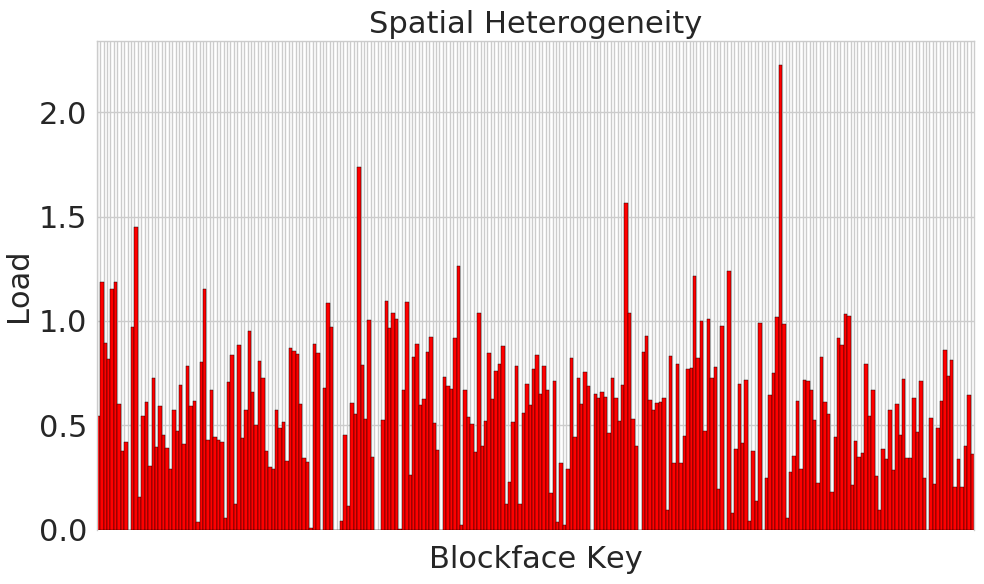
\includegraphics[width=.99\textwidth]{../figs/spatial_heterogeneity.png}
\caption{Spatial heterogeneity plot of the Belltown neighborhood.}
\label{fig:subim1}
\end{subfigure}\hfill
\begin{subfigure}[t]{0.45\textwidth}
\centering
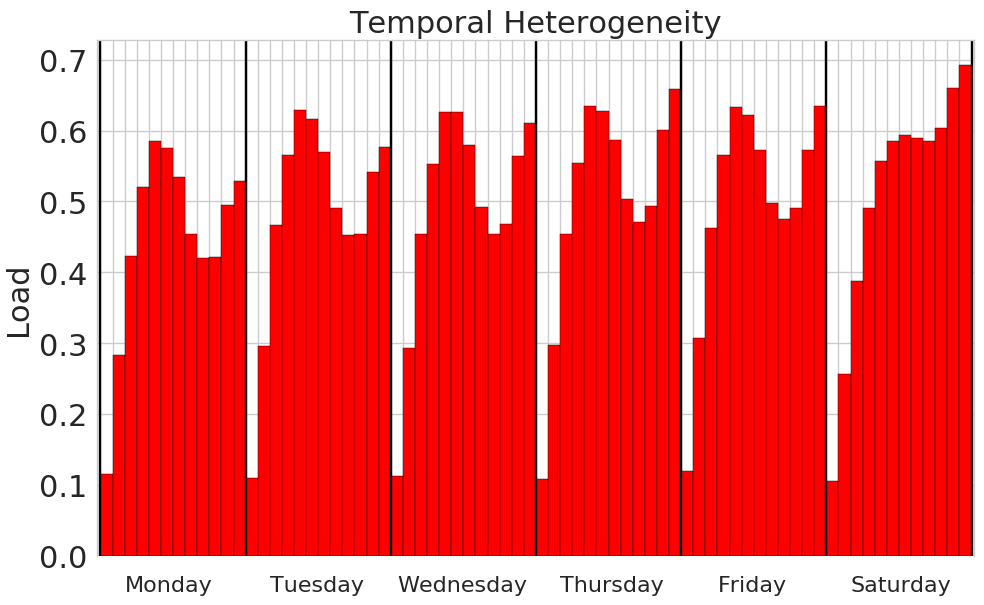
\includegraphics[width=.99\textwidth]{../figs/temporal_heterogeneity.png}
\caption{Temporal heterogeneity plot of the Belltown neighborhood.}
\label{fig:subim2}
\end{subfigure}
\caption{}
\label{fig:image2}
\end{figure}

\noindent
The spatial heterogeneity demonstrated in figure 1a, is one of the fundamental reasons that using average occupancy as the sole factor in policy decisions is an insufficient metric when considering how occupancy impacts congestion. The temporal heterogeneity demonstrated in figure 1b, shows that parking behavior is similar during weekdays, while behavior on Saturdays is very different. These properties of parking behavior are key when designing control strategies to mitigate congestion. We further observe that within the Belltown neighborhood there are centers of demand that dictate a majority of the congestion. The centers of demand are repeatable at given time of day and day of week over time, and we also find that the centers of demand change with time of day and day of week. We model locational demand by using a Gaussian Mixture Model (GMM) with spatial and occupancy data.

\section{Gaussian Mixture Model for Locational Demand Analysis}
As discussed previously, the occupancy of parking exhibits spatial heterogeneity within the Belltown neighborhood. By using a GMM we can identify centers of demand based on spatial information and occupancy data. By first considering only the occupancy data we can begin to get an idea for the distribution of parking occupancy and how parking behavior changes over the course of a day.

\begin{figure}[H]
\begin{subfigure}[t]{0.45\textwidth}
\centering
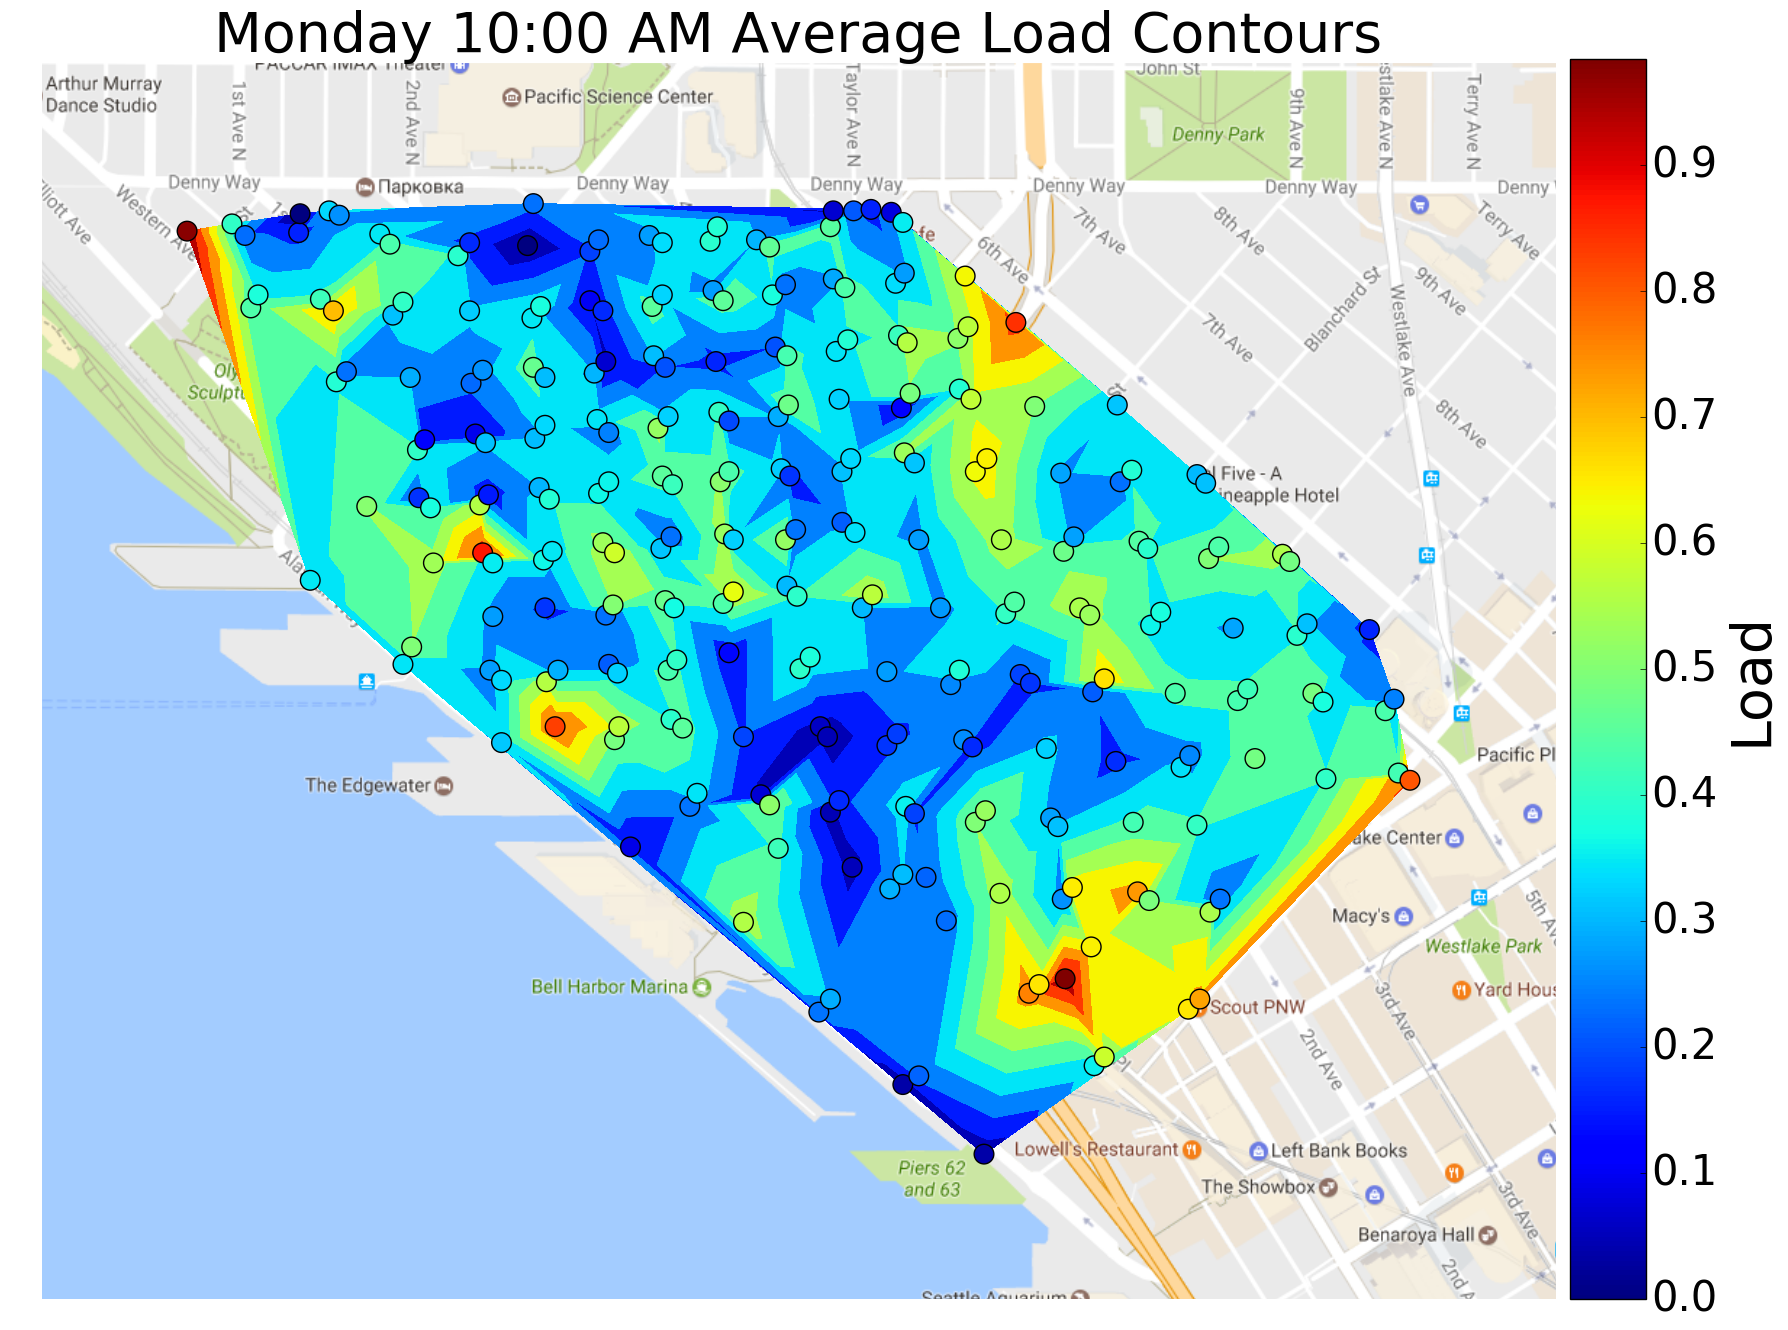
\includegraphics[width=.99\textwidth]{../figs/monday_10am.png}
\caption{10 Contours of the average load in the Belltown neighborhood at 10:00 AM on Monday.}
\label{fig:subim1}
\end{subfigure}\hfill
\begin{subfigure}[t]{0.45\textwidth}
\centering
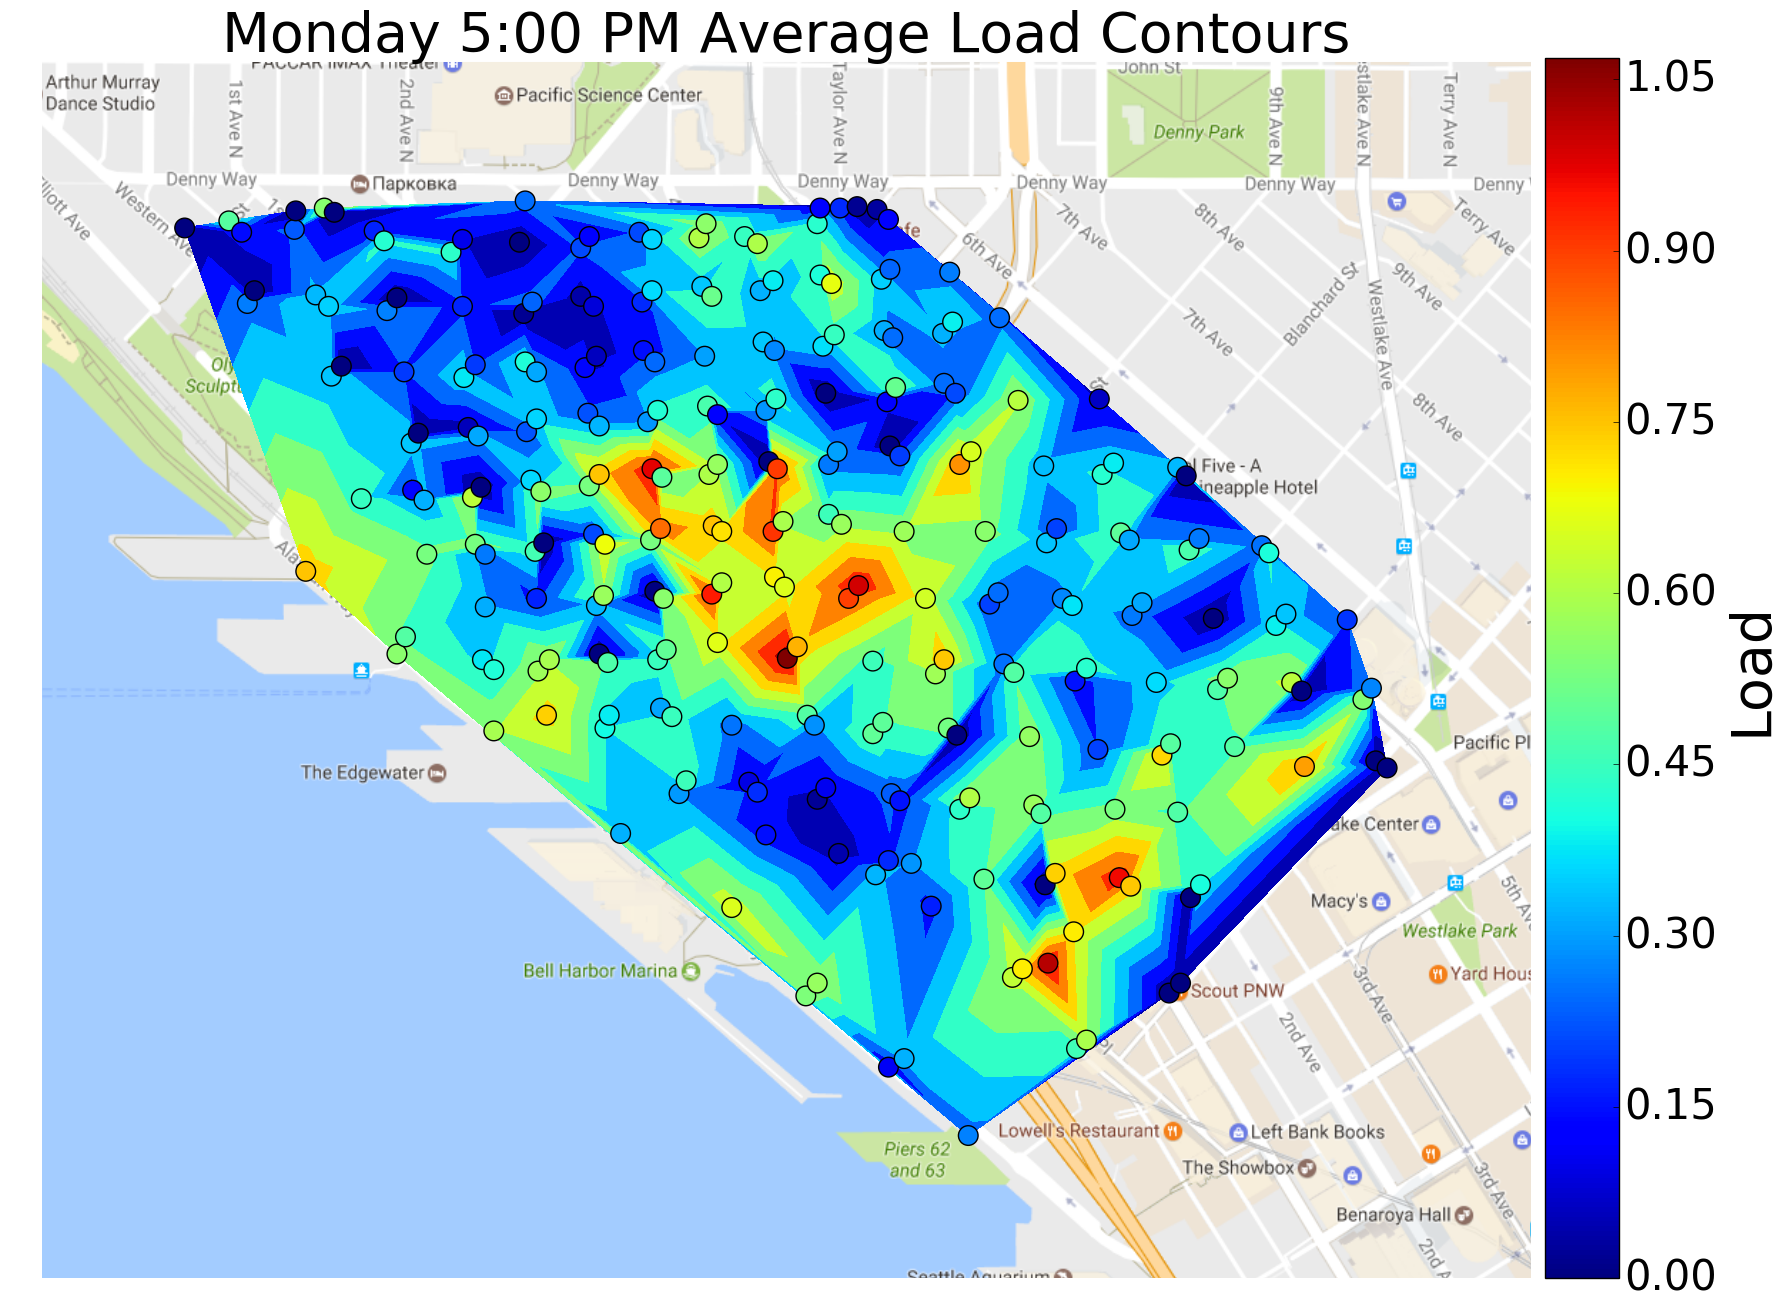
\includegraphics[width=.99\textwidth]{../figs/monday_5pm.png}
\caption{10 Contours of the average load in the Belltown neighborhood at 5:00 PM on Monday.}
\label{fig:subim2}
\end{subfigure}
\caption{}
\label{fig:image2}
\end{figure}

\noindent
Although in figure 1a it can be observed that across Belltown there is a similar average load on Monday at 10:00 AM and 5:00 PM, the contour plot reveals that locational demand changes over a course of a day. In the morning parking is spread more uniformly across the neighborhood as people arrive to work. In the evening the parking becomes much more concentrated in the center of the neighborhood where many of the popular restaurants and bars are located.
\newline
\indent
Using a GMM we can model the centers of demand and give an estimate the influence the centers of demand have on neighboring blockfaces. A GMM can be used as an unsupervised clustering method to find partitions in a population containing similar samples. We consider a Multivariate GMM in which each sample $\bar{x}_i$ is a vector containing spatial and occupancy data as $\bar{x}_i = [x_{\text{latitude}}, \ x_{\text{longitude}}, \ x_{\text{load}}]$. The purpose is to find which of the K possible mixture components each sample belongs to with the highest probability. Each mixture component has a prior on the probability of a sample belonging to it, $P(C_j) = \pi_j$. The likelihood of a sample belonging to a mixture component is then given as a Multivariate Gaussian Distribution 
\begin{equation}
P(\bar{x}_i|C_j) = \frac{1}{(2 \pi)^{\frac{3}{2}}|\Sigma|^{\frac{1}{2}}}
e^{-\frac{1}{2}(\bar{x}_i - \bar{\mu}_j)^T\Sigma_j^{-1}(\bar{x}_i - \bar{\mu}_j)}.
\end{equation}
We assume that the features $(x_{\text{latitude}}, \ x_{\text{longitude}}, \ x_{\text{load}})$ are conditionally independent given the component, i.e. each covariance matrix $\Sigma_j$ is diagonal. The GMM is a classic chicken and the egg problem. We want to find the component that each sample belongs to, but to do so we need to know the distributions of each of the components. This problem is solved by the expectation-maximization (EM) algorithm which maximizes the log likelihood of the data. In the EM algorithm we initialize each of the component parameters, i.e. the prior, mean, and covariance, randomly. Until convergence is reached, which occurs when the complete log likelihood given by $L = \sum_{i=1}^n log \sum_{j=1}^k P(C_j)P(\bar{x}_i|C_j)$, increases by an amount smaller than some $\epsilon$, two steps are repeated at each iteration of the algorithm. These are the E step, in which the expected values of the unobserved component labels are calculated with the current parameter values, and the M step, in which new parameter values are calculated to maximize the probability of the data. The E step for all samples $x_i$ is
\begin{equation}
P(C_j|\bar{x}_i) = \frac{P(C_j)P(\bar{x}_i|C_j)}{\sum_{i^{'}}P(C_{i^{'}})P(\bar{x}_i|C_{i^{'}})}
\end{equation}
and the M step for all components is
\begin{equation}
P(C_j) = \frac{1}{n}\sum_{i=1}^nP(C_j|\bar{x}_i) 
\end{equation}
\begin{equation}
\bar{\mu}_i = \frac{\sum_{i=1}^n\bar{x}_iP(C_j|\bar{x}_i)}{\sum_{i=1}^n P(C_j|\bar{x}_i)} 
\end{equation}
\begin{equation}
\Sigma_j = \frac{\sum_{i=1}^n(\bar{x}_i - 
\bar{\mu}_j)^2P(C_j|\bar{x}_i)}{\sum_{i=1}^n P(C_j|\bar{x}_i)}.
\end{equation}
At convergence each sample $x_i$ is assigned the component label which maximizes the posterior probability $P(C_j|\bar{x}_i)$, and the component parameters are recorded. 
\newline
\indent
The GMM also involves a model selection problem in selecting the appropriate number of mixture components. We used both the Akaike Information Criterion (AIC) and the Bayesian Information Criterion (BIC) when choosing the model, whose equations are given as follows.
\begin{equation}
\text{AIC} = -2\text{ln}(L) + 2k
\end{equation}
\begin{equation}
\text{BIC} = -2\text{ln}(L) + \text{ln}(n)k
\end{equation}
In each of these models, $L$ is the maximized log likelihood of the GMM, $n$ is the number of data points used in the GMM, and $k$ is the degrees of freedom in the GMM. In a GMM containing $C$ components with three dimensional data, there are seven degrees of freedom for each component. Three degrees of freedom come both the diagonal covariance matrix and the mean vector, and the final degree of freedom comes from the mixing weight. In total the number of parameters for the complete GMM is then $k = 7 \cdot C$.
\begin{figure}[H]
\begin{subfigure}[t]{0.45\textwidth}
\centering
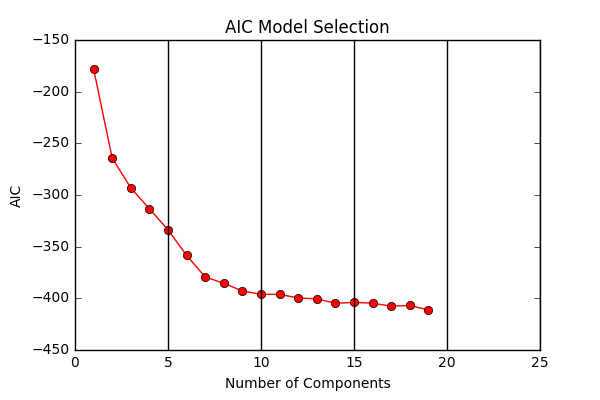
\includegraphics[width=.99\textwidth]{../figs/aic_model.png}
\caption{Akaike information criterion for model selection.}
\label{fig:subim1}
\end{subfigure}\hfill
\begin{subfigure}[t]{0.45\textwidth}
\centering
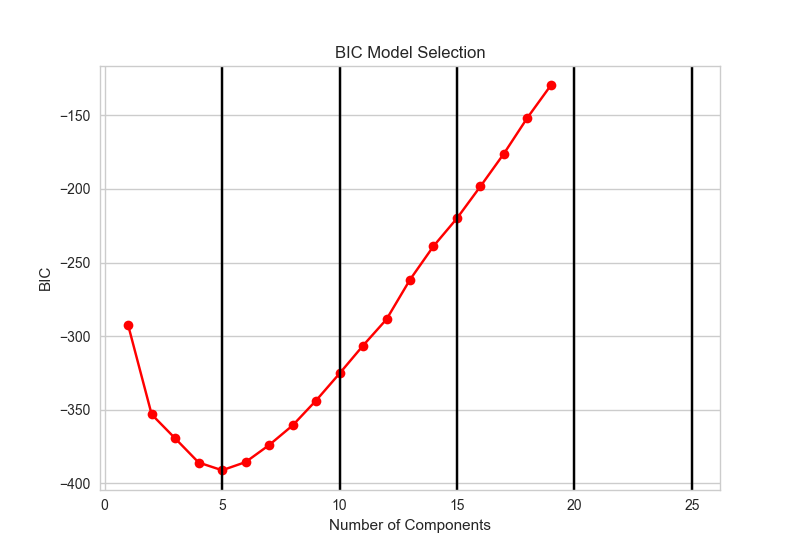
\includegraphics[width=.99\textwidth]{../figs/bic_model.png}
\caption{Bayesian information criterion for model selection.}
\label{fig:subim2}
\end{subfigure}
\caption{}
\label{fig:image2}
\end{figure}
\noindent
The AIC is known to often select a more complex model than the BIC. For this reason we considered both criterion and chose to use four components in our model.
\begin{figure}[H]
\begin{subfigure}[t]{0.45\textwidth}
\centering
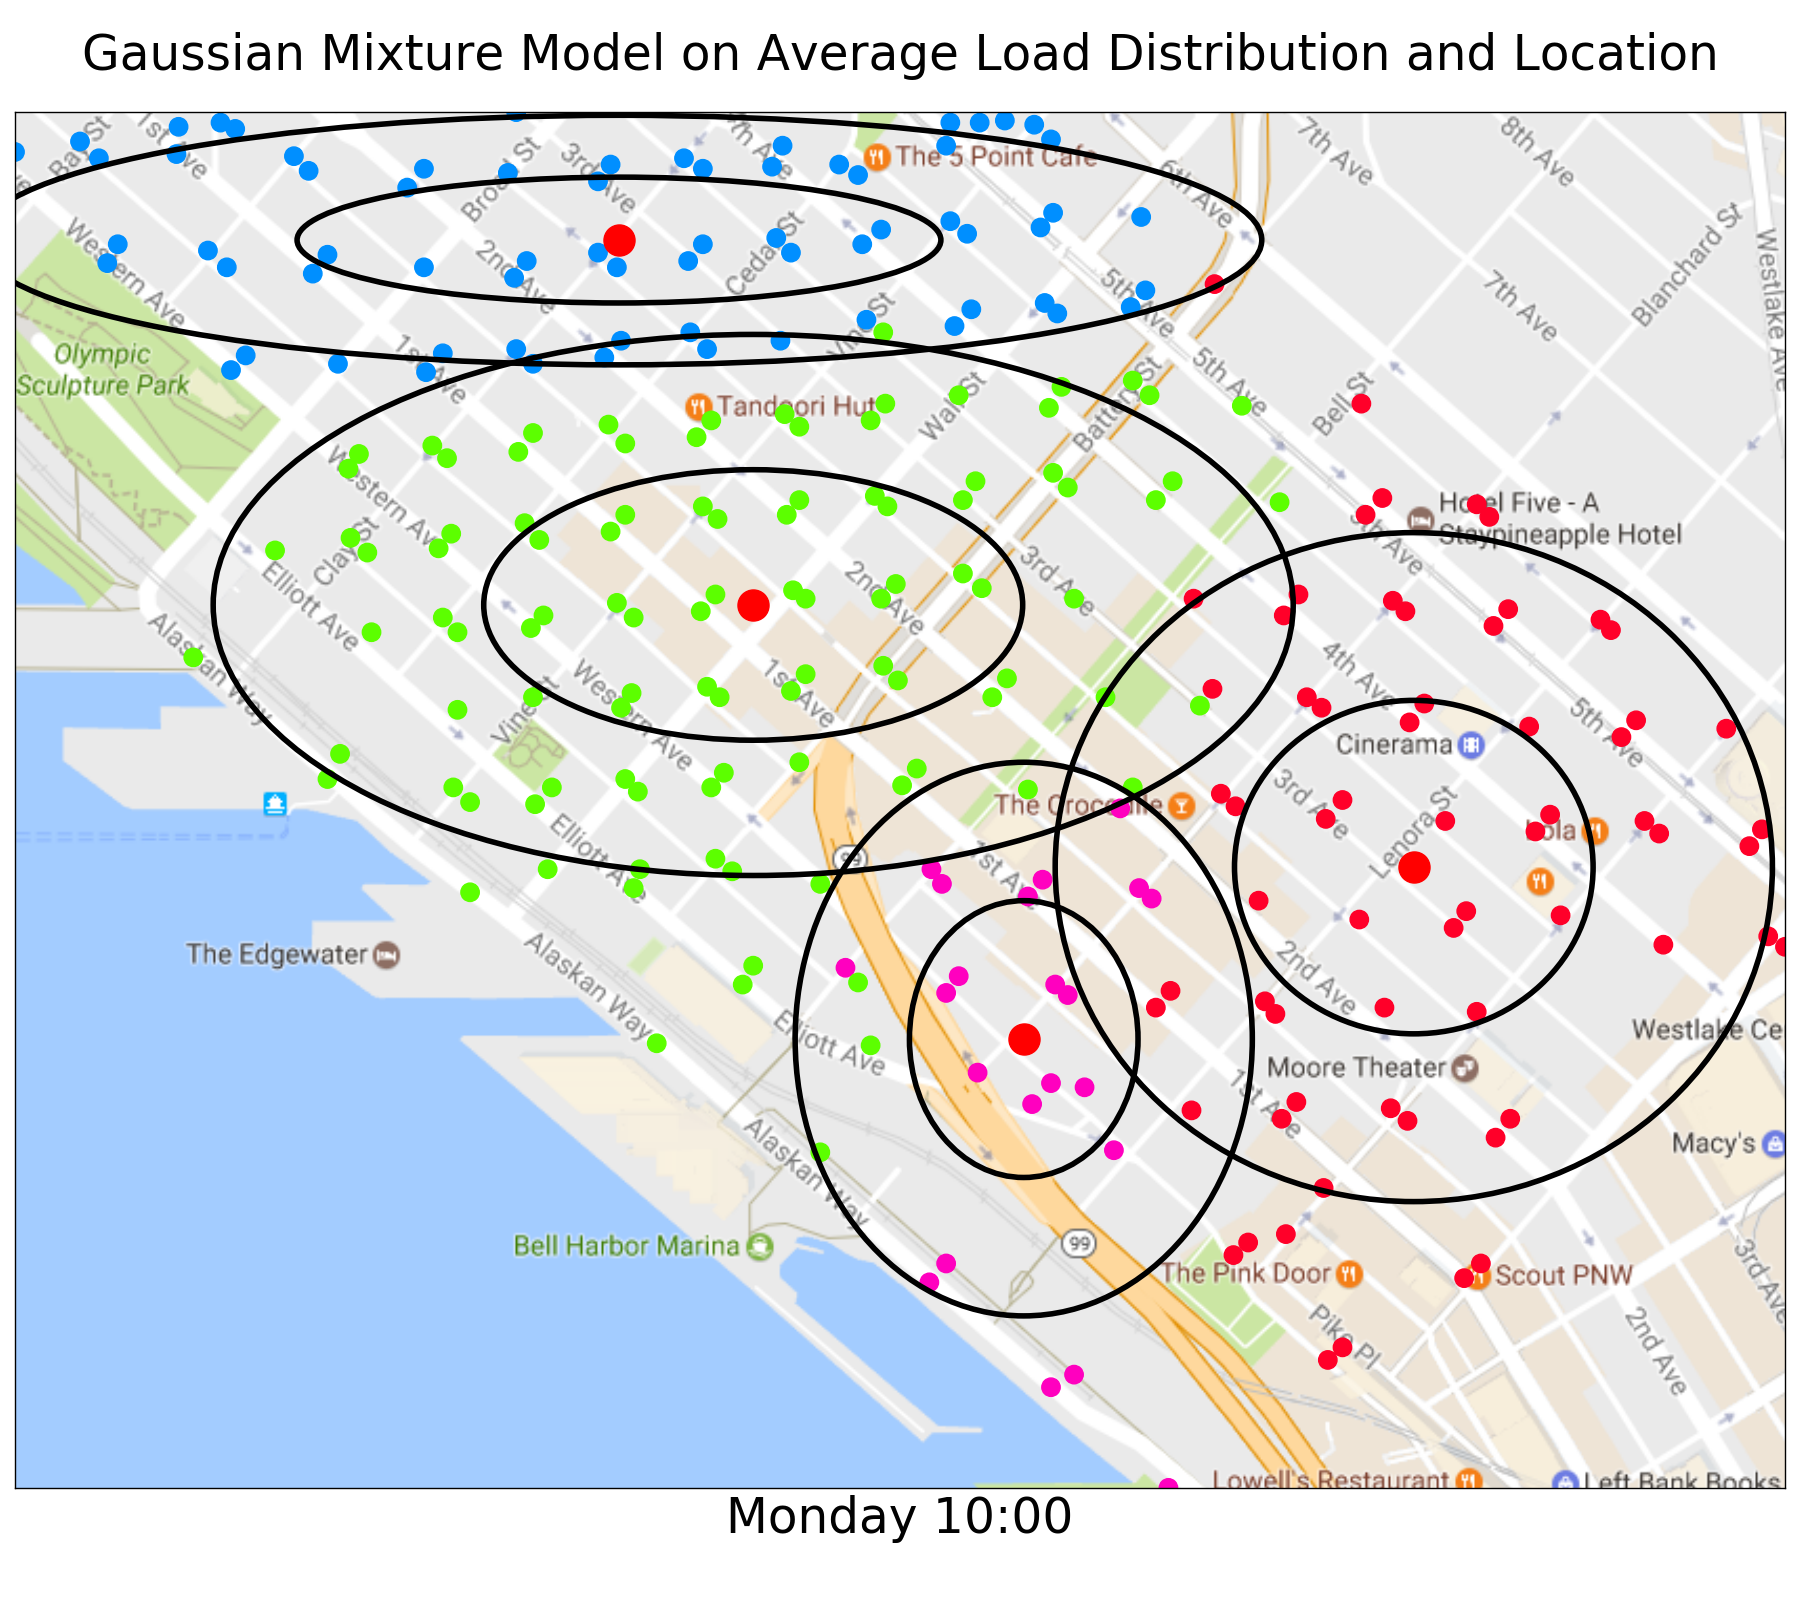
\includegraphics[width=.99\textwidth]{../figs/monday_10am_gmm.png}
\caption{GMM applied to the Belltown neighborhood at 10:00 AM on Monday.}
\label{fig:subim1}
\end{subfigure}\hfill
\begin{subfigure}[t]{0.45\textwidth}
\centering
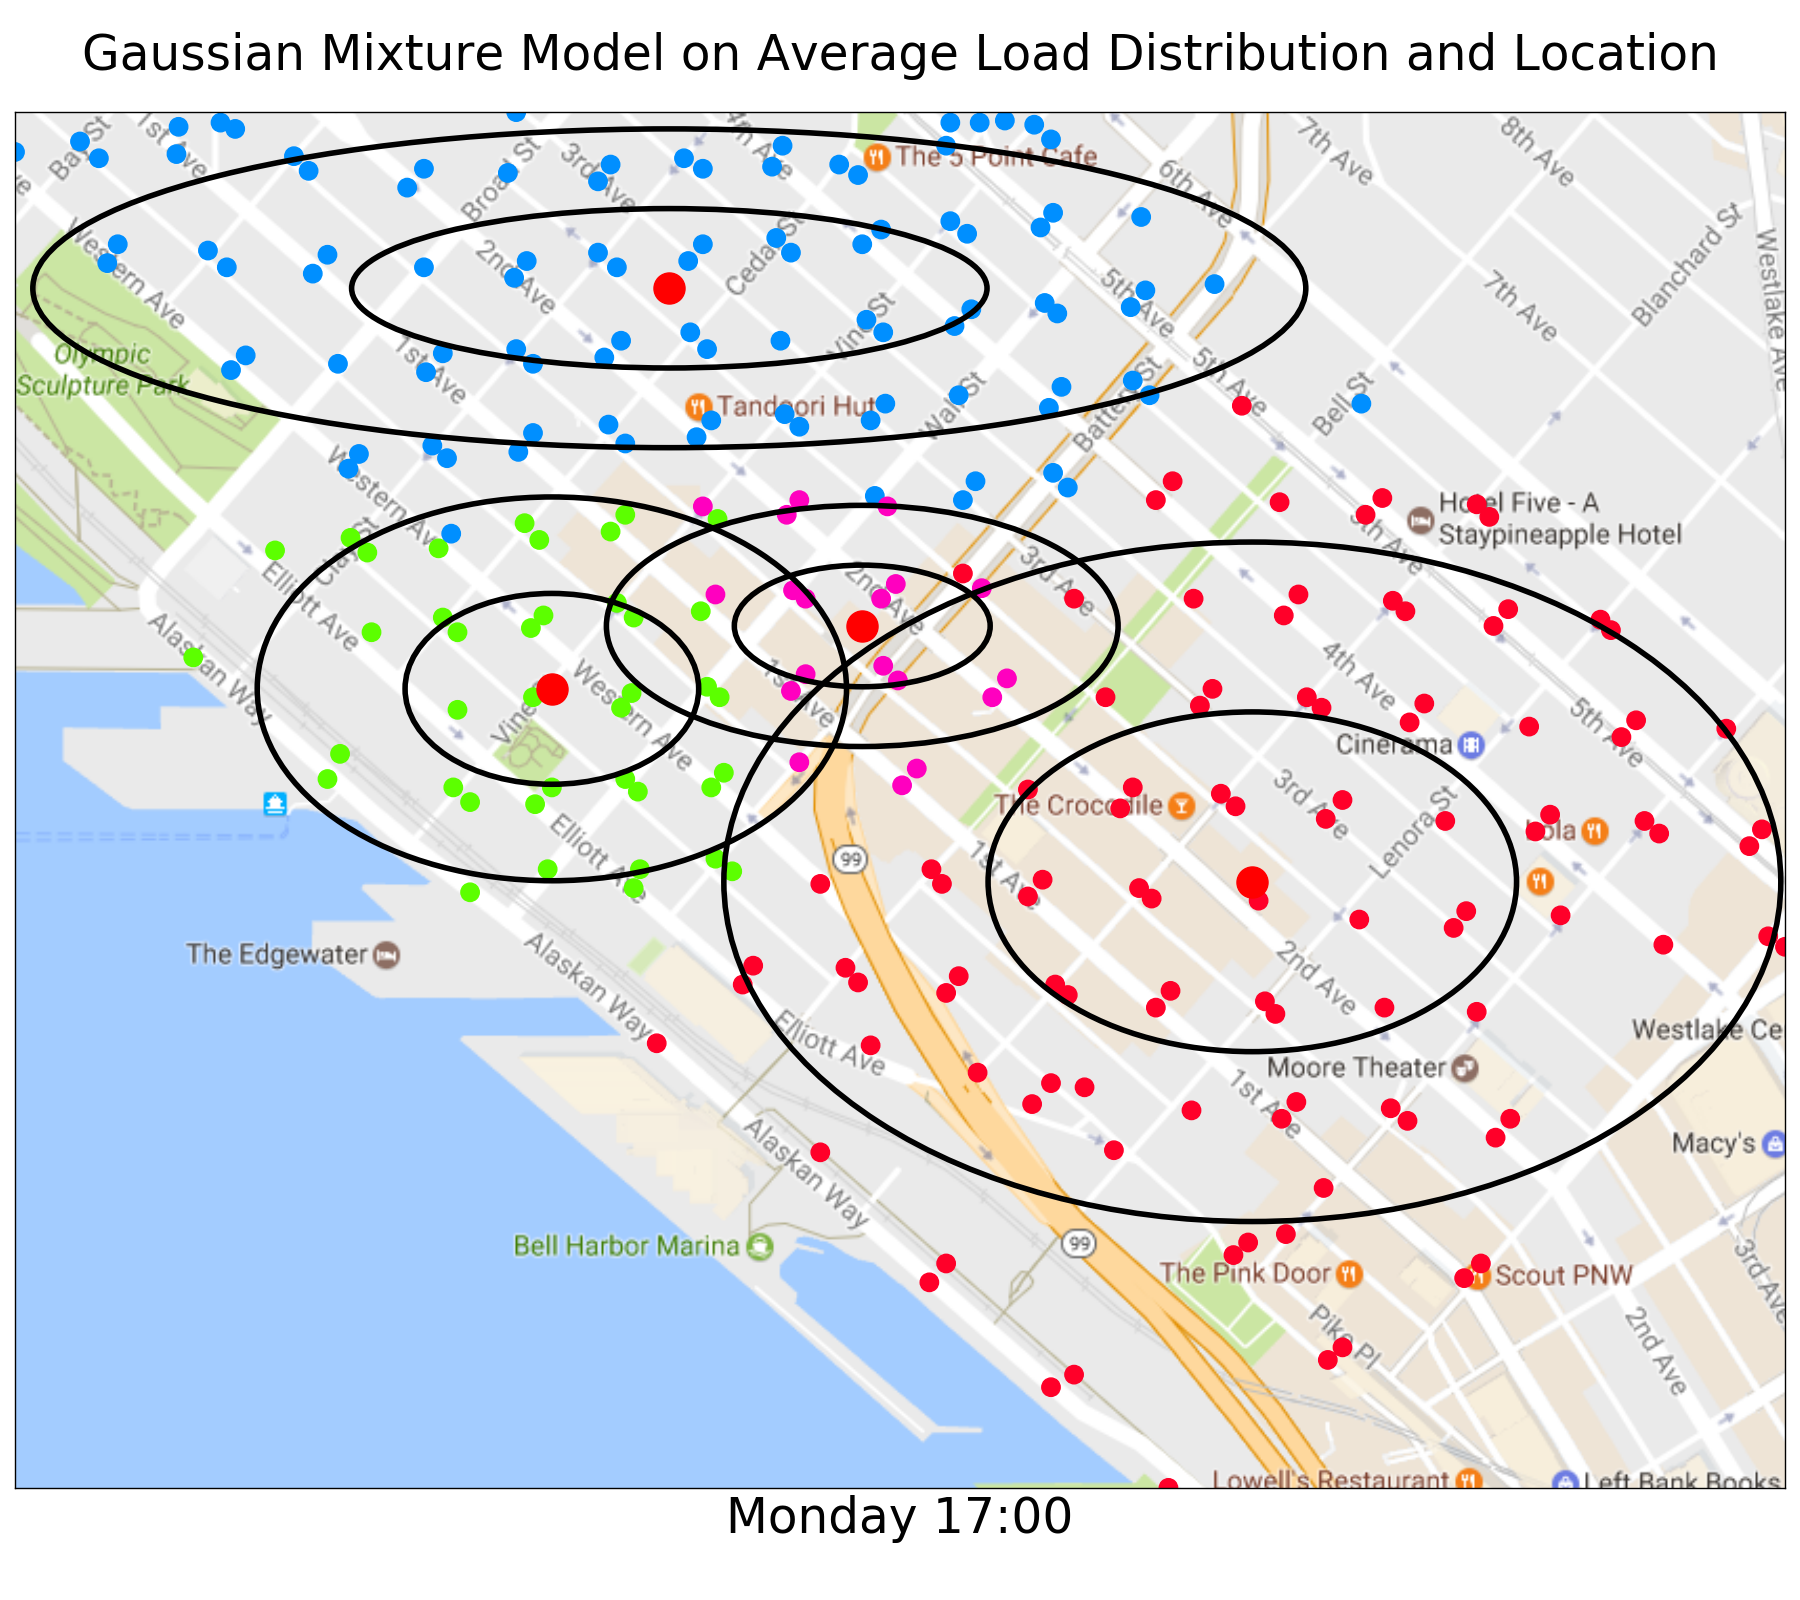
\includegraphics[width=.99\textwidth]{../figs/monday_5pm_gmm.png}
\caption{GMM applied to the Belltown neighborhood at 5:00 PM on Monday.}
\label{fig:subim2}
\end{subfigure}
\caption{}
\label{fig:image2}
\end{figure}


% \begin{figure}[H]
% \centering
% 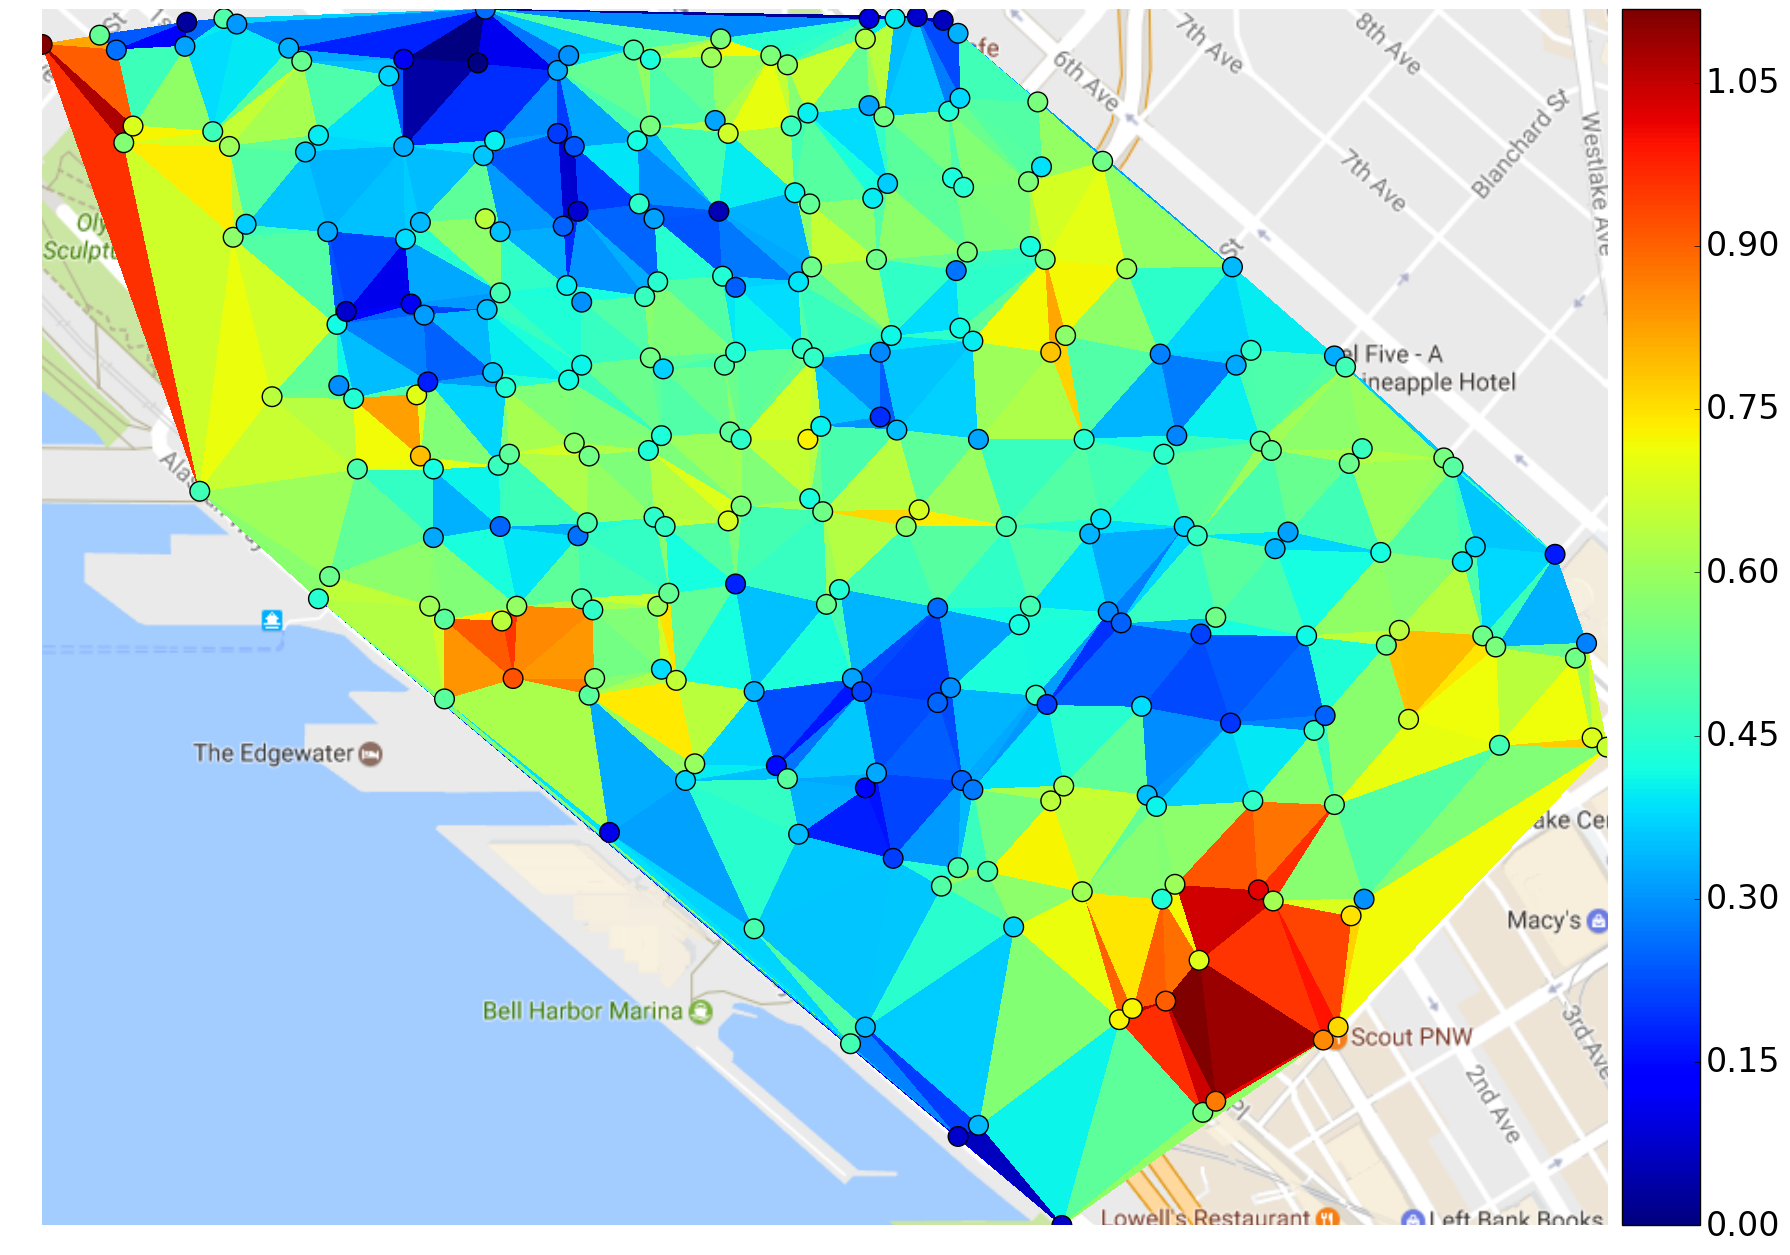
\includegraphics[height=8cm, width=8cm, keepaspectratio]{../figs/triangle.png}
% \caption{Triangle plot of the Belltown neighborhood.}
% \end{figure}

% \begin{figure}[H]
% \centering
% 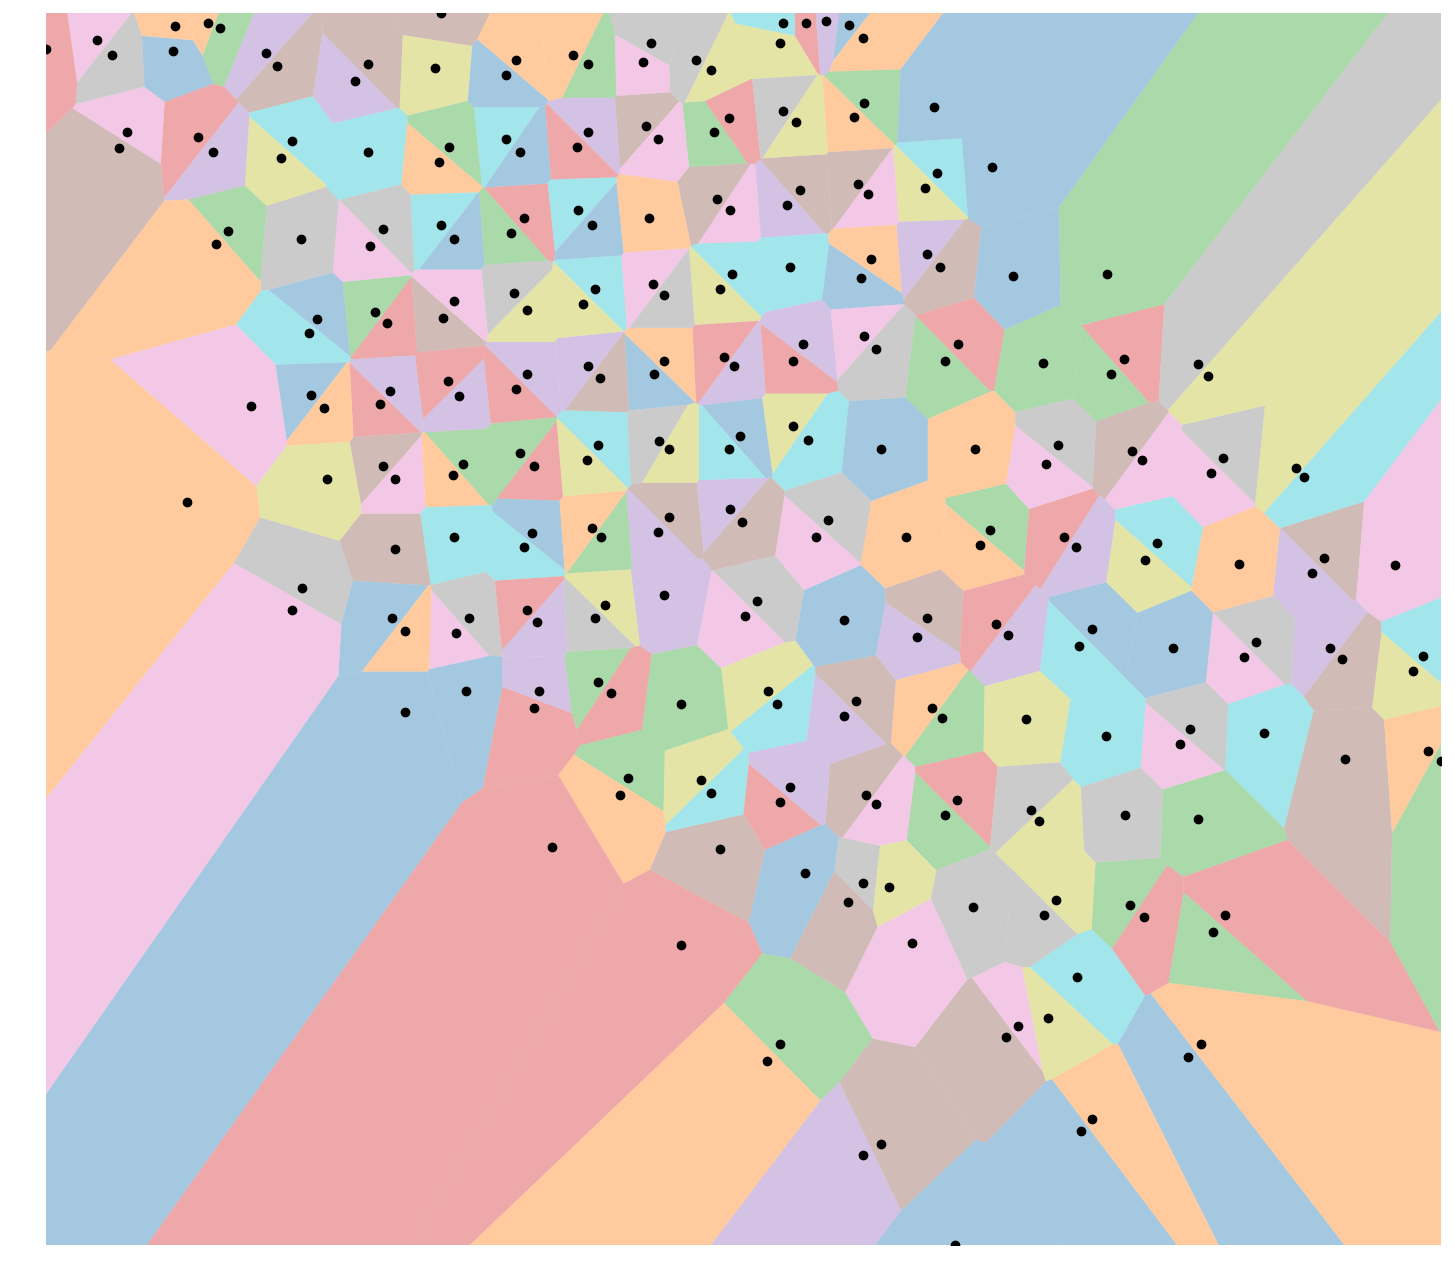
\includegraphics[height=8cm, width=8cm, keepaspectratio]{../figs/voronoi.png}
% \caption{Voronoi diagram of the Belltown neighborhood.}
% \end{figure}

% \begin{figure}[H]
% \centering
% 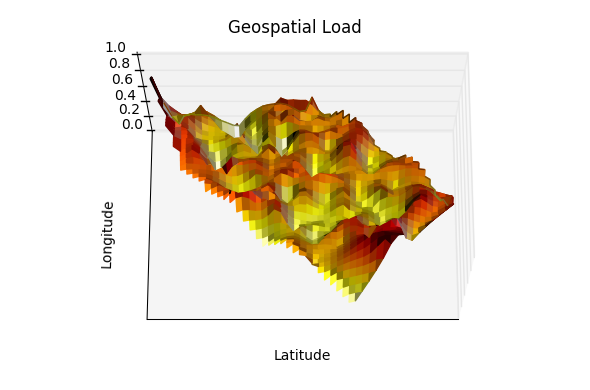
\includegraphics[height=8cm, width=8cm, keepaspectratio]{../figs/surface.png}
% \caption{Surface plot of the Belltown neighborhood.}
% \end{figure}



\end{document}